\documentclass[a4paper, 10pt]{report}
\usepackage[italian]{babel}
\usepackage[T1]{fontenc}
\usepackage[utf8]{inputenc}
\usepackage{charter}
\usepackage{amsmath}
\usepackage{amsthm}
\usepackage{amsfonts}
\usepackage{graphicx}
\usepackage{wrapfig}
\usepackage{tcolorbox}
\usepackage{fancyhdr}
\usepackage{listings}
\usepackage{longtable}

\usepackage{geometry}
\geometry{a4paper, left=2cm,right=2cm,top=2cm,bottom=2cm}

\pagestyle{fancy}
\lhead{}
\chead{}
\rhead{\bfseries 09 ottobre 2019 }
\lhead{\bfseries Segnali e immagini}

\begin{document}

\section*{\underline{Tassonomie per segnali}}

Un segnale è una funzione generica $f: D_1 \rightarrow D_2$ che associa ad ogni elemento del dominio $D_1$ uno ed un solo elemento del dominio $D_2$. I due domini possono essere sottoinsiemi degli Interi, Reali o Complessi; gli elementi dei dei due domini possono essere scalati, vettori ($[0 1 2]$) oppure matrici. 

Il tipo di segnale generato è vincolato al tipo di dominio e codominio, come rappresentato dalla seguente figura:

\begin{center}
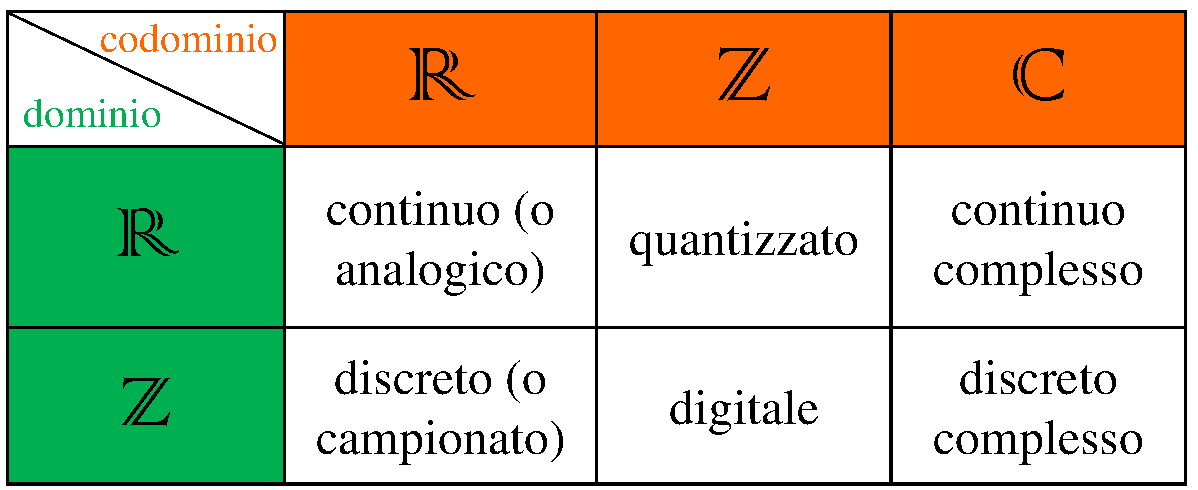
\includegraphics[scale=0.3]{24_cropped.pdf}
\end{center}

\noindent In base a cosa rappresentano i segnali, ovvero dove varia la variabile indipendente, abbiamo:
\begin{itemize}
\item[-] Segnali temporali (variazione nel tempo);
\item[-] Segnali spaziali (variazione nello spazio);
\item[-] Segnali frequenziali (variazione nelle frequenze).
\end{itemize}

\begin{center}
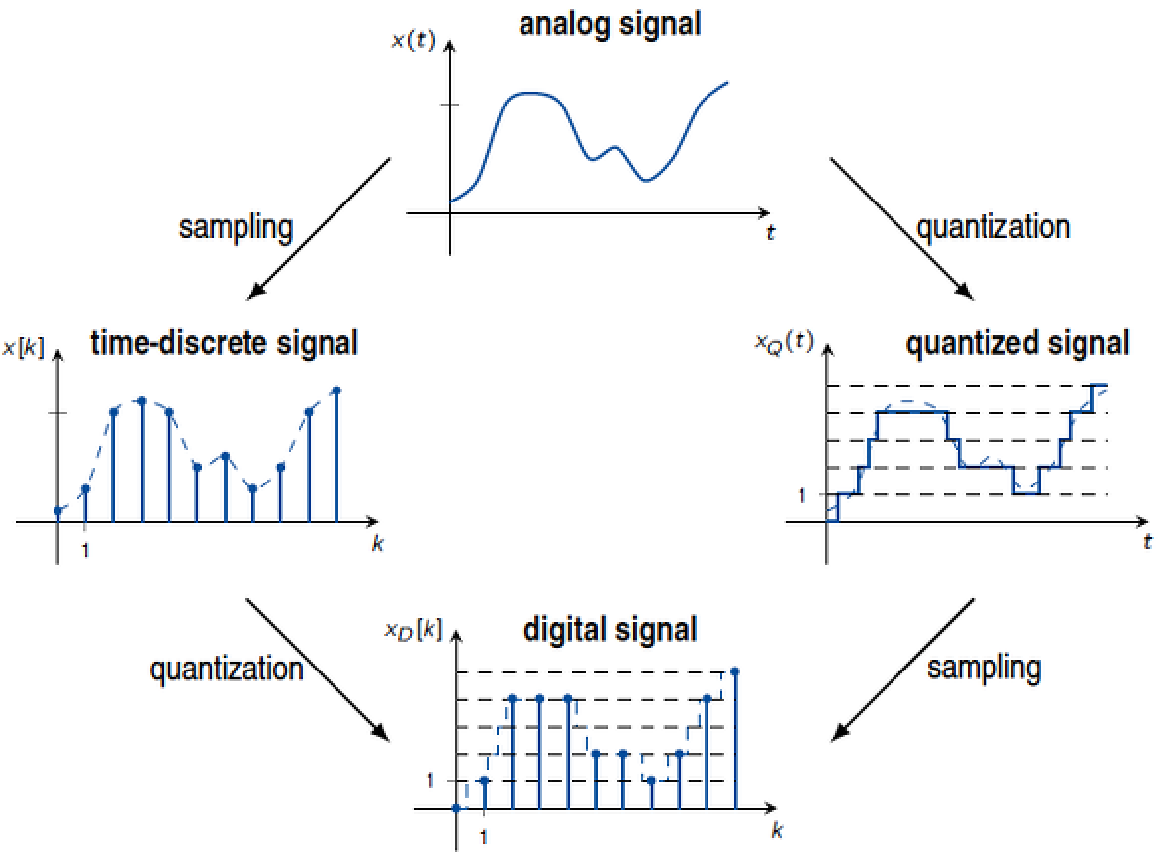
\includegraphics[scale=0.4]{25_cropped.pdf}
\end{center}

\begin{tcolorbox}[title=\textbf{Fasore}]
Un fasore è una funzione complessa di variabile reale che modella la posizione di un punto che ruota attorno all'origine con raggio $|c|$ e velocità angolare costante $\theta(t)$.

Il fasore permette di passare dal dominio del tempo/spazio a quello dell'analisi frequenziale.

Un fasore fa variare nel tempo un numero complesso (in forma polare) mantebebdone il modulo $|c|$ fisso:
\begin{align*}
|c|e^{j \theta} -> |c|e^{j \theta(t)}
\end{align*}

$\theta (t)$ (velocità angolare) indica l'angolo spazzato a partire da un angolo $\phi$ ad un certo istante $t$. Si può calcolare con la seguente formula:
\begin{align*}
\theta (t) = \frac{2 \pi}{T_0} t  + \phi
\end{align*}

dove $T_0$ indica il tempo necessario a spazzare $2 \pi$ radianti.
\end{tcolorbox}

\subsection*{Categorie di segnali}

\begin{longtable}{| p{.15\textwidth} | p{.80\textwidth} |}
\textbf{Segnali temporali continui} & il dominio $D_1$ è sottoinsieme dei numeri reali; la variabile indipendente rappresenta il tempo. Se:
\begin{itemize}
\item[-] $D_1 = R(-\infty, +\infty)$, il segnale è "a tempo continuo";
\item[-] $D_1 = R[0, +\infty)$, il segnale è "causale continuo";
\item[-] $D_1 = R(t_start, t_end)$, il segnale è "ad intervallo limitato continuo";
\end{itemize}

Solitamente il codominio è $D_2 = R[VAL_min, VAL_max]$, ovvero il segnale è limitato.\\\\

\textbf{Segnali spaziali continui} & il dominio $D_1$ è sottoinsieme dei numeri reali e costituito di matrici; la variabile indipendente è rappresentata attraverso 2 coordinate (tempo e spazio). Generalmente $D_1 = R(t_start, t_end) x R(z_start, z_end)$. Si tratta quindi di segnali "a supporto limitato continuo".

Il codominio può avere "dimensione" variabile ($R^n$).\\\\

\textbf{Segnali frequenziali continui} & il dominio $D_1$ è sottoinsieme dei numeri reali; la variabile indipendente rappresenta la frequenza ($\mu$), misurata in Hz ($secondi^{-1}$). Si tratta di segnali duali a quelli temporali/spaziali.

Il codominio $D_2$ è sottoinsieme dei numeri complessi ed è esprimibile attraverso due segnali: ampiezza e fase. Comunque, di solito si restringe il codomio ai numeri reali (la variabile y prende il nome di magnitudo). 

Per esprimere le proprietà dei segnali temporali/sequenziali attraverso segnali frequenziali è necessario ricorrere all'analisi di Fourier.

\begin{center}
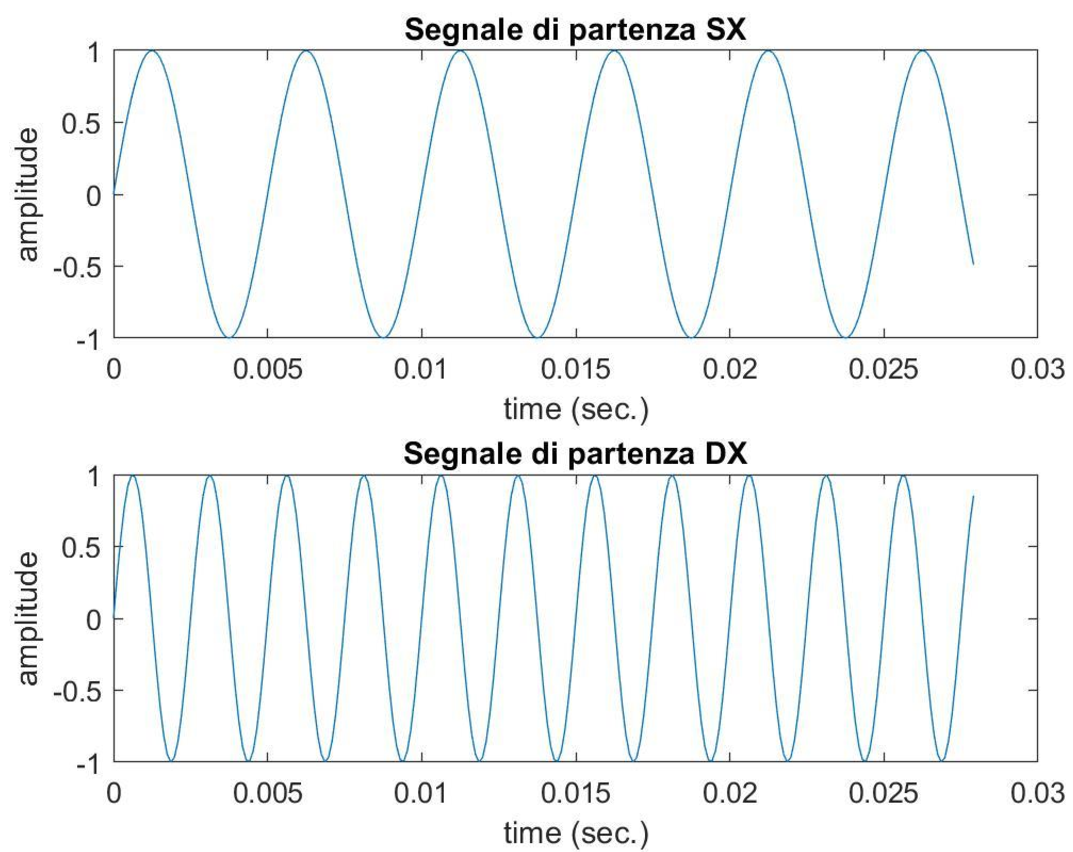
\includegraphics[scale=0.4]{34_cropped.pdf}
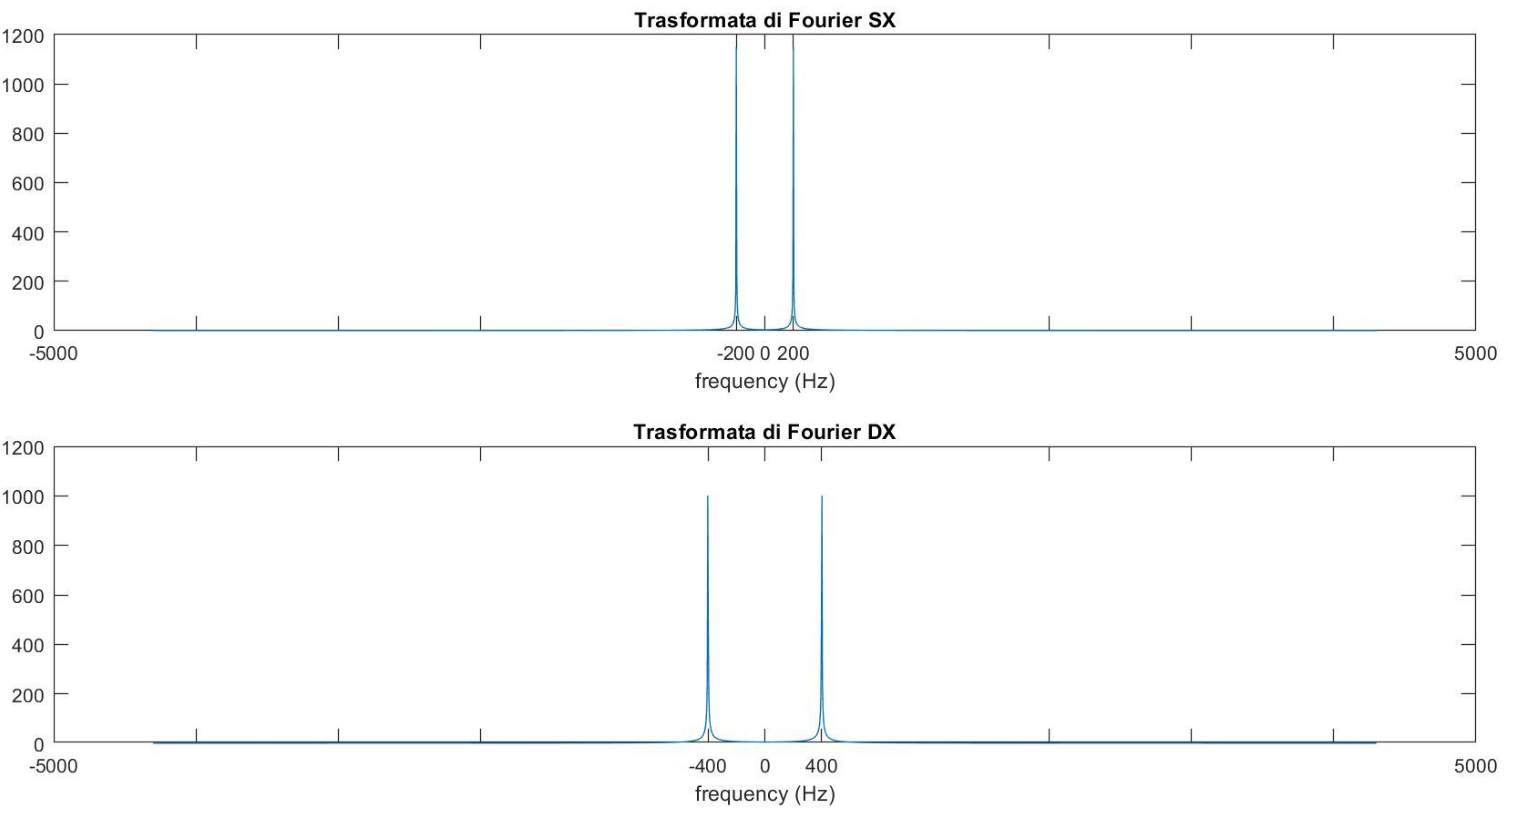
\includegraphics[scale=0.4]{35_cropped.pdf}
\end{center}

\noindent Tramite la Trasformata di Fourier, i segnali frequenziali descrivono il contenuto frequenziale del segnale.
\\
\hrule & \hrule
\\
\textbf{Segnali discreti} & Un segnale viene detto discreto quando il suo dominio viene campionato da un insieme discreto di punti ($D_1 \subset Z^{n_1(x n_2 ...)}$), dove il dominio è $D_1 = \{..., t_{-3}, t_{-2}, t_{-1}, t_0, t_1, t_2, t_3, ...\}$ con i vari $t$ equidistanti. I segnali discreti possono essere di qualsiasi natura (temporali, spaziali, frequenziali).

Esempio: $D_1 = \{..., -3, -2, -1, 0, 1, 2, 3, ...\}$. 

Sono segnali discreti, ad esempio, una stringa di DNA, un segnale audio preso ad istanti prefissati, un'immagine rappresentata tramite pixel (i pixel sono indicizzati spazialmente ad intervalli fissi).

Quando i segnali discreti derivano da una
decimazione del dominio della variabile
indipendente si parla di campionatura, o
segnale campionato.

Attenzione: anche i segnali discreti possono essere analizzati in frequanza.
\\
\hrule & \hrule
\\
\textbf{Segnali digitali} & I segnali digitali sono segnali discreti le cui ampiezza sono quantizzate (es: canzione mp3, immagine nel pc).

Attenzione: anche i segnali discreti possono essere analizzati in frequanza.
\\
\hrule & \hrule
\\
\textbf{Segnali periodici} & Un segnale $f$ è detto periodico, con periodo $T$, se:
\begin{center}
$ \exists T \in R^+$ tale che $f(t + T) = f(t)$,  $\forall t \in D_1$
\end{center}

\noindent e $T$ è il minor numero per cui la condizione ri ripetizione si verifica.

Dato un periodo $T$, si indica con $\mu_0$ la "frequenza fondamentale" $\mu_0 = 1/T$.

\paragraph*{Segnali periodici trigonometrici} Fissato un $T>0$, i segnali trigonometrici di minimo periodo $T$ sono:
\begin{center}
$f(t) = cos2\pi \mu_0 t$ \hspace{1cm} $f(t) = sin\pi \mu_0 t$
\end{center}

\noindent Spesso si ha che $2\pi \mu_0 = 2\pi / T = \omega_0$, che rappresenta la velocità angolare (o pulsazione). 

Fissato un $\theta \in R$ (\textbf{fase}), è possibile eseguire operazioni di shift, in quanto il segnale originale (uno dei due sopra) e la versione con sommato $\theta$ nella parentesi hanno lo stesso periodo $T$.
\end{longtable}

\subsection*{Energia e potenza di un segnale}

\paragraph*{Energia} L'energia $E_f$ di un segnale si definisce come segue:
\begin{align*}
\begin{cases} 
\int_{-\infty}^{+\infty} f^2(t)\, dt & $se$ f \in R \\\\
\int_{-\infty}^{+\infty} |f(t)|^2\, dt & $con$ |f(t)|^2 = f^*(t)f(t)$,  se $f \in C
\end{cases} 
\end{align*}

\noindent Un segnale si dice ad energia finita (o di energia)  se l'integrale che ne rappresenta l'energia converge ad un valore diverso da 0 (oppure l'ampiezza va a 0). Si misura in joule.

Sono segnali di energia gli impulsi rettangolari e $sinc$; non lo sono $sin$ e $cos$.

Se un segnale è ad energia finità allora esiste la sua trasformata di Fourier (se non è ad energia finita, potrebbe esistere comunque la trasformata).

\paragraph*{Potenza media} La potenza media $P_f$ di un segnale si definisce come segue:
\begin{align*}
\begin{cases} 
lim_{T \to +\infty} \frac{1}{T} \int_{-T/2}^{+T/2} f^2(t)\, dt & $se$ f \in R \\\\
lim_{T \to +\infty} \frac{1}{T} \int_{-T/2}^{+T/2} |f(t)|^2\, dt & $con$ |f(t)|^2 = f^*(t)f(t)$,  se $f \in C
\end{cases} 
\end{align*}

\noindent Un segnale si dice a potenza finita (o di potenza) se l’integrale che
ne rappresenta la potenza converge ed è diverso da 0.

Per un segnale ad energia finita la potenza tende a zero (per cui un
segnale non può appartenere ad entrambe le categorie):

Esistono comunque segnali che non appartengono a nessuno dei due tipo sopra.

\end{document}